\begin{figure*}[!htp]
	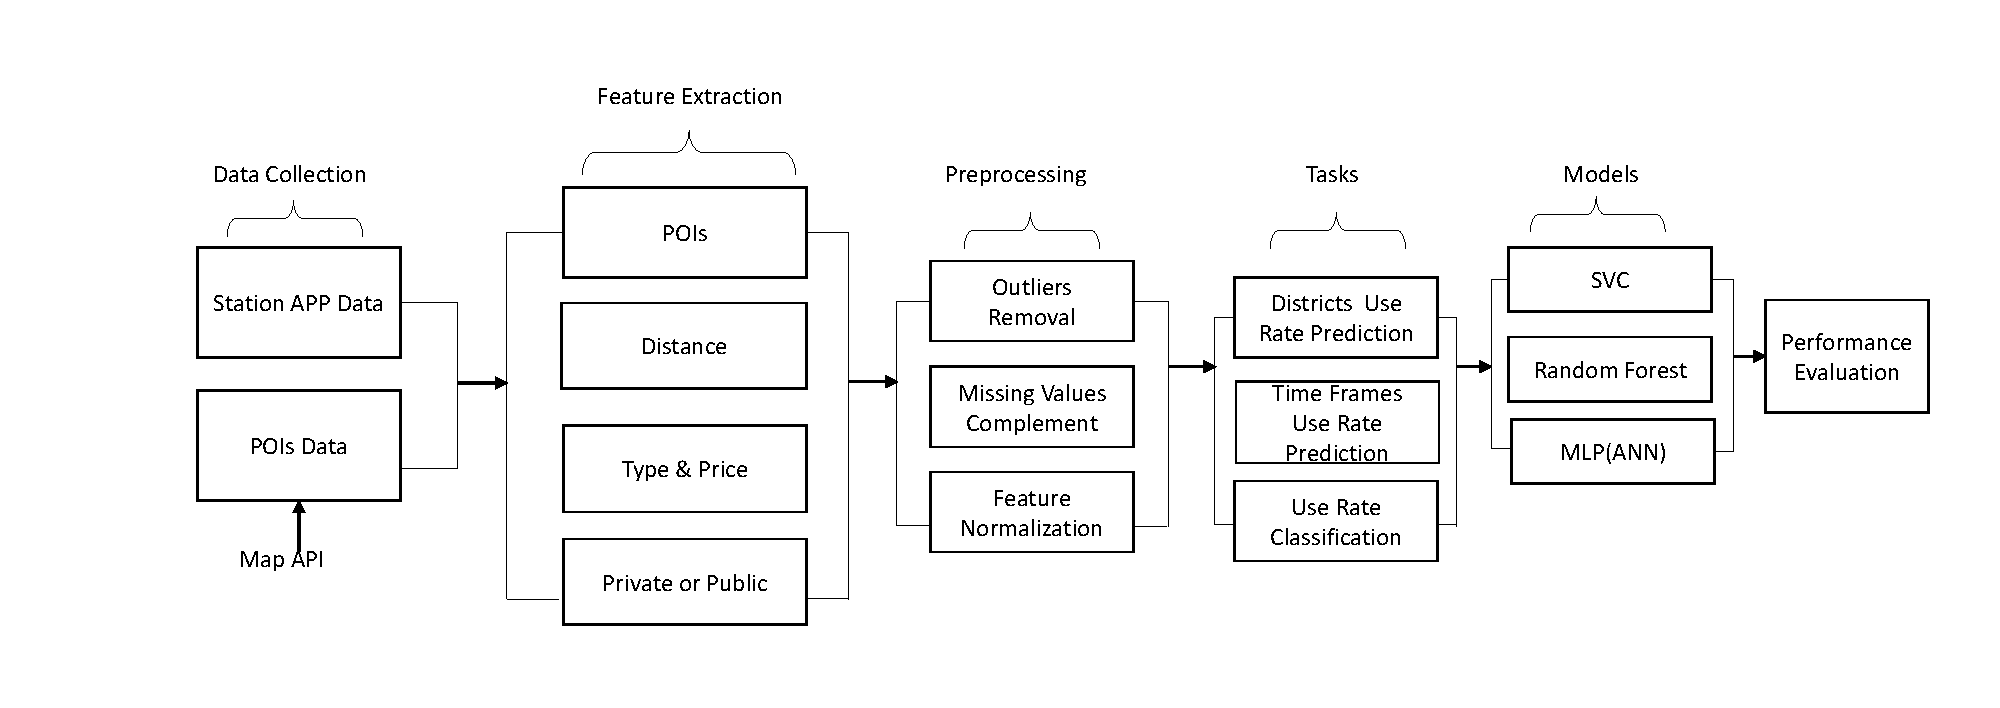
\includegraphics[width=2\columnwidth]{./figures/pipeline.pdf}
	\centering
	\caption{Overall Pipelines of Data Processing and Learning}
	\label{fig2}
\end{figure*}

Hence, we studied the optimization problem of how to deploy charging stations. Existing works \cite{Bao:2017,Liu:2018:DSB,Yang:2016:MMP,Li:2018:DBR,Liu:2016:RB} mainly fall into the domain of bike-sharing. The objective is to find a proper strategy for bike lane planning or sharing-bikes reposition, in order to help with a more resonable city planning. \cite{Bao:2016,Chen:2011,Jiang:2016,Li:2016}, they are usually based on sharing-bikes' trajectory data, which is full of spatio temporal information. \cite{Bao:2017} provides a data-driven apporoach to deal with bike lane construction problem. It takes government constraints of planning bike lanes, such as budget limitations, construction convenience and bike lane utilization into consideration to formulate the problem. Furthermore, the problem is proved to be NP-hard so that they propose a greedy network expansion algorithm to help work out a scalable and approximate solution to bike lane planning problem. The approach performs well in the given problem, however it doesn't make use of learning models. \cite{Li:2018:DBR} introduces a reinforcement learning algorithm to help solve the problem of repositioning sharing-bikes. First it uses an inner-balance clustering algorithem to cluster stations into groups, then the reinforcement learning algorithm is conducted in each group to learn a reposition policy. They make a good use of spatio-temporal data while don't take advantages of useful surrounding and station-self features. \cite{Liu:2016:RB} proposes a new method using weighted K-Nearest-Neighbor to predict bike-sharing stations' pick up demand and a new model to predict drop off demand, it also study on stations clustering to simplify the problem. With these steps they explore a useful way to optimize bike-sharing system's rebalancing operations.

Current works of location selection are usually based on the flow prediction of a single station. Futhermore, they rely heavily on the historical data. \cite{Yang:2016:MMP} introduces a model for bicycle mobility prediction. It relis on historical bike-sharing data and a per-station basis with sub-hour granularity. It makes use of the randonm forest prediction model to implement their experiments and obtain a rather good result. \cite{Liu:2016:CTP} gives an optimization to this problem. Its way for traffic prediction no longer focuses on the history data only, but can use location-based socail media to collect a much larger area of the traffic data for predicting traffic conditions. Other work on urban life prediction take advantages of spatio temporal data and useful machine learning algorithms \cite{Hoang:2016,Li:2018,Liao:2018:DSL:3219819.3219895,Liu:2016:CTP,Shen:2018:SNS,Zhou:2018:DLP:3219819.3219929}. \cite{Zhou:2018:DLP:3219819.3219929} make use of users' geographical check-in information in Wechat and dig into the rich spatio temporal representations behind users' activity at cultural venues. Then the authors propose a latent Dirichlet allocation model to identify latent patterns of urban cultural interactions, in order to help with urban cultural planning and investment optimazation. \cite{Shen:2018:SNS} is also a good example of prediction model for spatio-temporal mobility event. It encodes each POI's spatio and temporal dependencies rather than neglect the correlations between POIs. 

In this paper, we also focus on stations' spatio temporal data and make use of machine learning algorithms to help with our analyses. We argue that the surrounding point of interests(POIs), distances to important POIs(e.g, metro stations, estates, etc.), station charging price, AC/DC station types as well as whether a station is private of public for use, play important roles in selecting the optimal location for stations.
